\chapter{Alcance y diseño}
\label{ch:chap03}

\section{Alcance}
\label{sec:alcance}

\section{Proceso de desarrollo}
\label{sec:procdes}

Dada la naturaleza del proyecto, fue deseable establecer una metodología de desarrollo para facilitar el proceso de seguimiento del progreso incluso cuando el equipo de desarrollo fue individual.

Para ello, internamente, se utilizó una metodología ágil de desarrollo similar a la conocida como \textit{Kanban}.

Los principios claves del método aplicado a este proyecto fueron:
\begin{itemize}
	\item La visualización sencilla del curso de trabajo (una lista de tareas a realizar conocida como \textit{Backlog})
	\item La limitación de las tareas en progreso.
	\item Dirigir y gestionar el flujo de trabajo implica la priorización de tareas a realizar dada una cantidad finita de recursos.
\end{itemize}

La gestión de las tareas a relizar se llevó a cabo en el respositiorio del proyecto, con tareas como las vistas en \ref{img:kanban}. Donde se consideran un conjunto de tareas:

\begin{itemize}
	\item Backlog: Las tareas a realizar, en orden de importancia.
	\item In progress: Las tareas actualmente en desarrollo.
	\item Done: Las tareas cuya funcionalidad fue completamente desarrollada y probada.
\end{itemize}

\vspace{5mm}
\begin{minipage}[h]{0.8\linewidth}
	\centering
	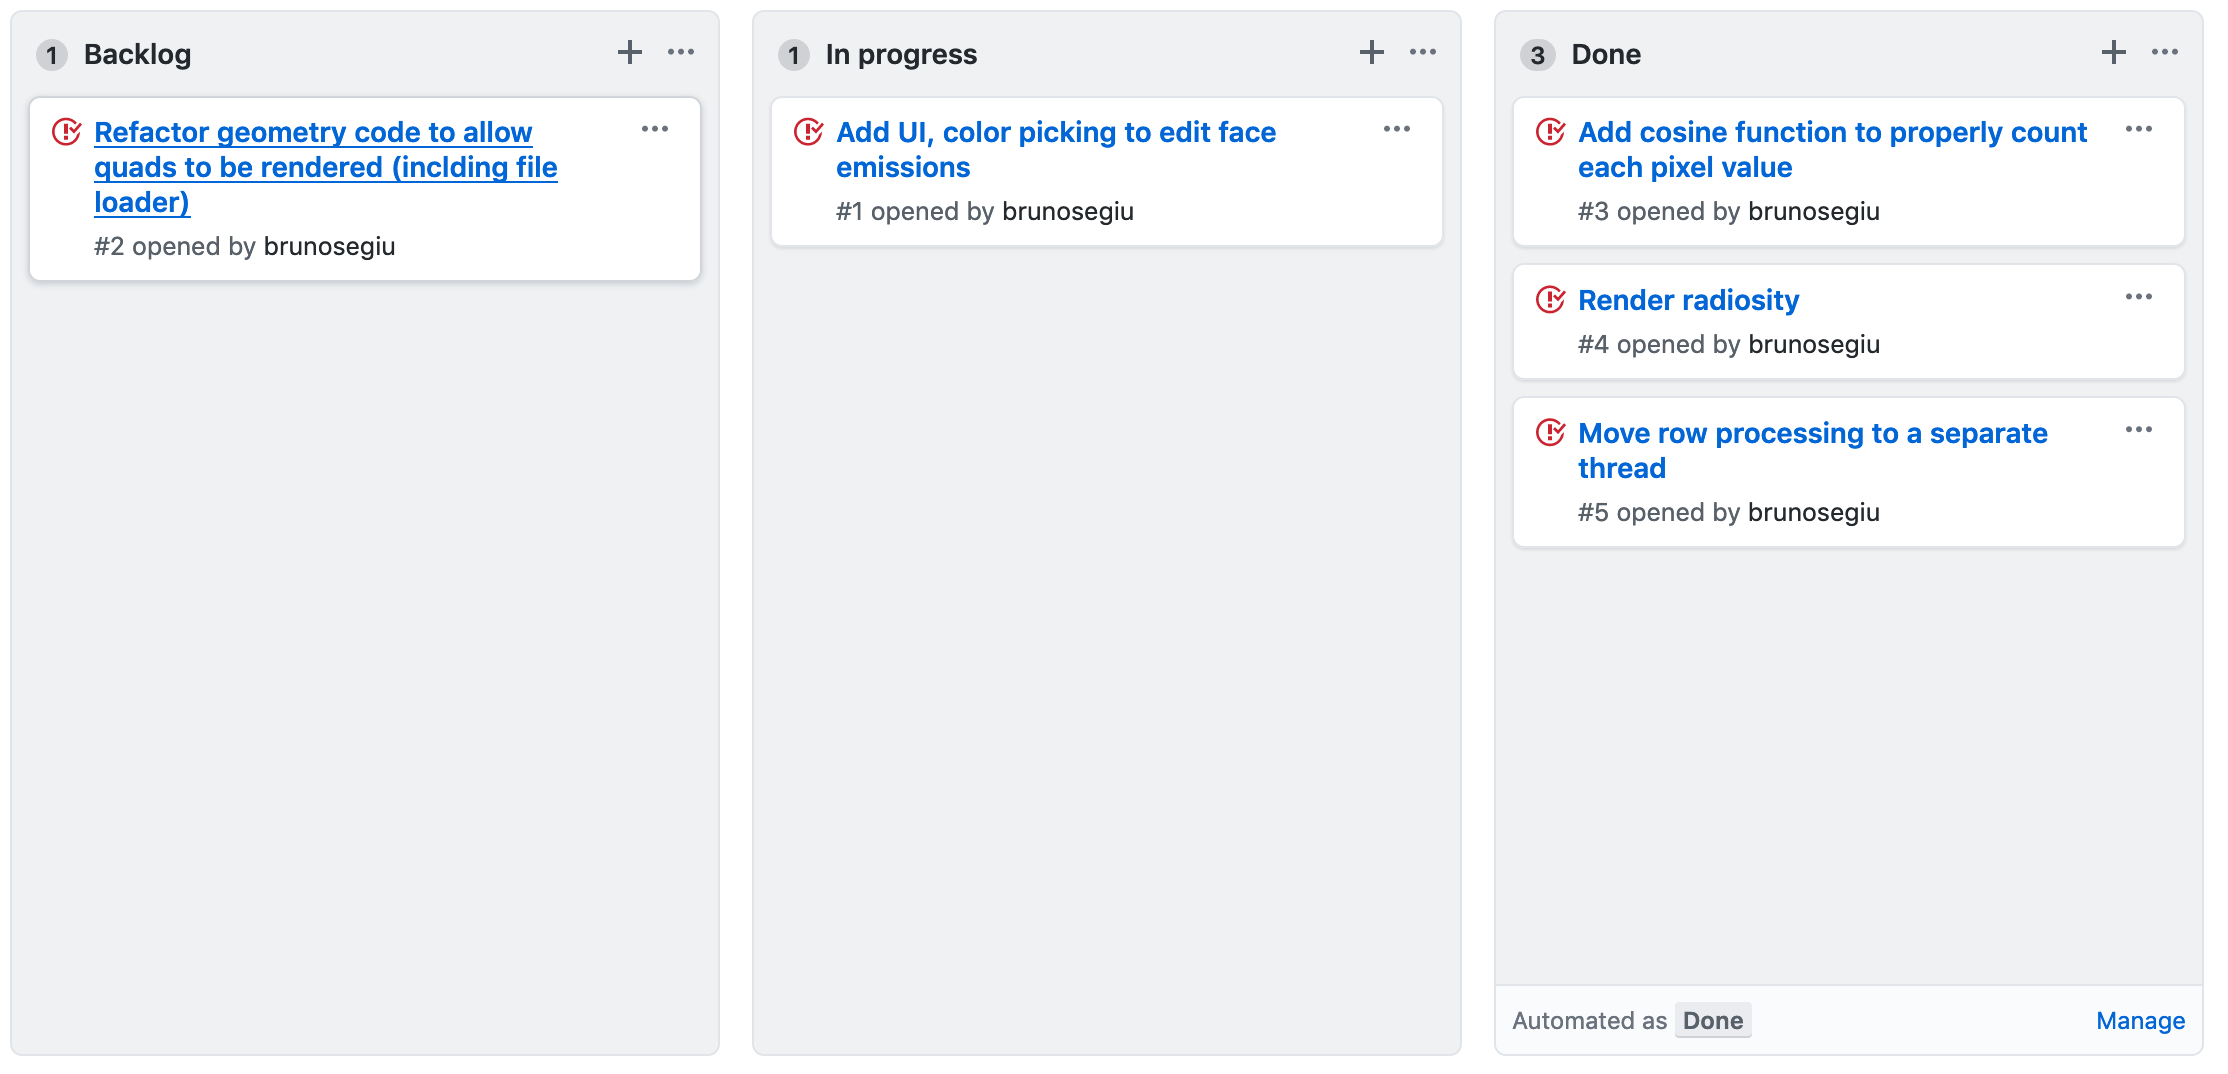
\includegraphics[width=\linewidth]{assets/kanban}
	\captionof{figure}{Tabla de Kanban utilizada en el proyecto}
	\label{img:kanban}
\end{minipage}

\section{Diseño}
\label{sec:disenio}

Con la finalidad de evitar el alto acoplamiento, facilitar la extensión y evitar errores de integración se tomó la decisión de utilizar distintos paquetes que ofrezcan un conjunto de funcionalidades.

El diseño de la solución comprende dos componentes principales, la interfaz gráfica de usuario (GUI, en inglés) y el motor de renderizado.

\subsection{Motor de renderizado}
\label{sec:engine}

El paquete del motor de renderizado se compone de un conjunto de módulos que manejan el pre-procesado de una escena, es decir, el cálculo de la radiosidad y el renderizado en tiempo real de la escena así como la carga de modelos desde el disco duro, la modificación de materiales, entre otras funcionalidades detalladas en \ref{sec:ui}.

\subsubsection{Módulo de pre-procesado}

El módulo de preprocesado se compone de un controlador principal, que maneja el estado y la ejecución de  los comandos de los distintos \textit{pipelines} implementados que resuelven el cálculo de la radiosidad.

Un pipeline es definido a partir de un conjunto de funciones ejecutadas en el siguiente orden:

\begin{enumerate}
	\item \verb|setConfig(scene, interpolator, reflections, n_channels, solver)|
	\item \verb|computeFormFactors()|
	\item \verb|computeRadiosity()|
\end{enumerate}

Donde \verb|computeFormFactors()| variará dependiendo del método de cálculo elegido, donde puede utilizarse el método del hemi-cubo o el de la hemi-esfera. El primero de ellos utilizará un \textit{pipeline} configurado utilizando una API de rasterización, mientras que el segundo utilizará una API capaz de calcular intersecciones utilizando \textit{trazado de rayos}.

La ejecución de \verb|computeRadiosity()| dependerá directamente de \verb|solver| seleccionará el algoritmo que calculará el vector de radiosidades para la escena.

\subsubsection{Módulo de visualización}

El módulo de visualización se encarga de renderizar la escena actual desde el punto de vista seleccionado por el usuario. Además, debe tener la capacidad de dibujar distintas propiedades de los materiales para facilitar la edición de las propiedades de los objetos o sus caras.

\subsubsection{Módulo de geometría}

El módulo de geometría procesa los archivos que contienen la información de la geometría de los modelos que componen la escena, los materiales y, la conversión y carga en memoria en formatos compatibles con las APIs de renderizado utilizadas.

\subsection{Interfaz gráfica}

El módulo de visualización (UI) utiliza una arquitectura basada en el paradigma del \textit{bucle de eventos} \ref{img:ui}, consiste en un bucle que detecta y maneja los distintos eventos recibidos por el sistema. Este método es útil para el manejo sencillo de la concurrencia en sistemas con múltiples hilos en ejecución y es de fácil implementación pues procesa cada uno de los eventos completamente antes de procesar el siguiente

En alto nivel, el \textit{bucle de eventos} se compone de la siguiente forma:

 \begin{lstlisting}[language=C]
 	while(queue.waitForEvent()){
 		queue.processEvent()
 	}
 \end{lstlisting}
 
 El  \textit{bucle de eventos} procesará todos los eventos de la aplicacación, lo que desencadena un conjunto de acciones que modificarán su \textbf{estado} de la interfaz de usuario. Este estado será dibujado por un conjunto de \textbf{componentes}, que no son más que presentadores del estado actual. Es decir, a partir de un conjunto de valores los presentarán en un formato gráfico adecuado y sencillo de comprender.

\vspace{5mm}
\begin{minipage}[h]{0.8\linewidth}
	\centering
	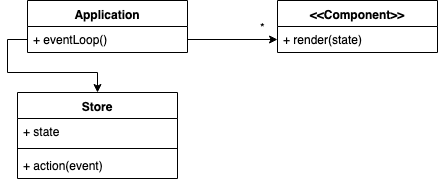
\includegraphics[width=\linewidth]{assets/ui}
	\captionof{figure}{Arquitectura general del módulo de interfaz de usuario}
	\label{img:ui}
\end{minipage}

\label{sec:ui}